% !TEX TS-program = pdflatexmk

\documentclass[a4paper, 12pt]{article}


% Include math
\usepackage{amsmath,amsthm,amssymb}
% Include links
\usepackage{hyperref}
%listings
\usepackage{listings}

%tocibind
\usepackage[nottoc]{tocbibind}


%%%%%%%%%%%%%%  PAGE SETUP %%%%%%%%%%%%%%%%%

\usepackage[margin=1.2in]{geometry}
\usepackage{float}
\usepackage{graphicx}
\usepackage[T1]{fontenc}
\usepackage{titling}
\usepackage{pdfpages}
\linespread{1.25}
\usepackage[toc,page]{appendix}
\usepackage[utf8]{inputenc}
\usepackage[english]{babel}

\usepackage{csquotes}
\usepackage[backend=biber,sorting=none]{biblatex}
\bibliography{citations}
\usepackage{caption}

\usepackage[utf8]{inputenc}
\usepackage[T1]{fontenc}
\usepackage{lmodern}
\usepackage{color}
\usepackage{hyperref}
\usepackage{epstopdf}
%\usepackage[table]{xcolor}
\usepackage{misc/matlab}
\usepackage[export]{adjustbox}

\hypersetup{colorlinks,linkcolor={blue},citecolor={blue},urlcolor={blue}}

\usepackage[framed,numbered,autolinebreaks,useliterate]{misc/mcode}
\usetikzlibrary{automata,positioning}

\setlength{\droptitle}{-10em}  

% The following sets up some headers
\usepackage{fancyhdr}
\setlength{\headheight}{52pt}
\pagestyle{fancy}
\lhead{Final report} % Left Header
\rhead{\thepage} % Right Header
\cfoot{} % Center Foot (empty)

% Document content begins here
\begin{document}
\definecolor{light-gray}{gray}{0.95}
\newcommand{\code}[1]{\colorbox{light-gray}{\texttt{#1}}}


\lstset{language=Matlab}
\lstset{
    extendedchars=False,
    literate = 
    *{~}{{$\neg$}}1
}

% Set up a title

\begin{titlepage}
    \centering
    \vfill
    \begin{Large}
        A report \\ on \vspace{0.8cm} \\
    \end{Large}
    \vfill
    \textbf{\Huge  Fuzzy control of an \\ \vspace{0.6cm} inverted pendulum system} \\
    \vspace{5cm}
    \Large{ \hfill Sashank Krishna S \hfill 2019A8PS0184P \hspace{2cm}} \hfill \\ \vspace{0.5cm}
    \Large{ \hfill Satwik Vats  \hfill 2019A8PS0194P \hspace{2cm}} \hfill \\ \vspace{0.5cm}
    \Large{ \hfill Aryan Balyan \hfill 2019A8PS0193P \hspace{2cm}} \hfill \\ \vspace{0.5cm}
    \vfill
\end{titlepage}

\eject

\tableofcontents

\eject

\section{Introduction}

Hello world
\section{Mathematical setup}

The inverted pendulum system could be modelled using the following equation: $$(I + ml^2)\phi'' + mgl sin(\phi) = mlx'' cos(\phi) $$
The linearized version of the same is given by: $$ (I + ml^2)\phi'' - mgl\phi = mlx'' $$

The model assumes that the pendulum system is a rigid body, and that there is no air resistance. More elaborate models can be formulated in case the factors will be of significance.

\pagebreak

The differential equations were converted into difference equations using central the central differencing approach. Both the non-linear and linear differential equations were converted into this form, but only the non-linear versino is presented below. The rest of this study uses the more accurate non-linear model as well. $$ \phi[i] = \frac{mlcos(\phi[i-1])(u[i]-2u[i-1]+u[i-2])+mglsin(\phi[i-1])dt^2}{I+ml^2}+2\phi[i-1]-\phi[i-2] $$

The initial conditions used correspond to zero inputs and a mild disturbance in $\phi$. If we simulate this model alone, we can see the inverted pendulum fall down, rise back up, and repeat the motion. \\

To make the situation more realistic, gaussian noise was also added to this value of $\phi[i]$. i.e., $\phi[i] = \phi[i] + N(0,\sigma^2)$ was performed. This model for noise is not that realistic, since it can be rather erratic. But if our system can be stabilized despite this level of noise, we should be fine. Furthermore, $\sigma$ can be controlled in the simulation environment. \\

The Pendulum parameters considered for this study are as follows: \cite{ref2}
\begin{center}
\begin{tabular}{ | c | c | }
	\hline
	Mass 			& 	200 g \\
	\hline
	Length 			&	30 cm \\  
	\hline
	Moment of Inertia	&	0.006 $kg m^2$ \\
	\hline
\end{tabular}
\end{center}
\section{PID controller}

The PID controller was implemented in the velocity form as shown: $$ du = K_{p}(\phi[i]-\phi[i-1]) + K_{i}\phi[i] + K_{d}(phi[i]-2phi[i-1]+phi[i-2])$$ 
$$u[i+1] =  u[i] + du $$

The PID coefficients used are shown below:
\begin{center}
\begin{tabular}{ | c | c | }
	\hline
	$K_{p}$ 		& 0.48	 \\
	\hline
	$K_{I}$		& -1.6	 \\  
	\hline
	$K_{d}$		& -0.025	 \\
	\hline
\end{tabular}
\end{center}

Negative coefficients were used because of the unstable nature of the system. The tuning was done by hand, first by trial and error, and then by manually tweaking the coefficients to improve performance. Approaches such as ZN tuning and Cohen-Coon tuning were not applicable since the system at hand is intrinsically unstable. \\

Tuning could have been done better by using genetic algorithms to guess a set of PID parameters, and then evolve them closer towards the optimal set of parameters. This however was not done due to the lack of time and expertise. 
\section{Fuzzy control algorithms}

Hello world
\section{Results and discussions}

Many different simulations were run and captured in video form. All the useful videos recorded can be found \href{https://drive.google.com/drive/folders/1YSsqFpuCf-zBKHXfOGs2zDYO57xDAOi-?usp=sharing}{here}. \\

The simulations were ran with gaussian disturbances being added in every timestep. Hence, two different runs of the same simulation would yield different results. On an average, the results are acceptable, but there are still times when the fuzzy controller isn't able to stabilize the system for higher disturbance levels. \\

Having given that disclaimer, results from one run of the PID and FLC simulations are shown below, in figs. \ref{fig:PID} and \ref{fig:FLC} respectively. 

\begin{figure}[h!]
    \centering
    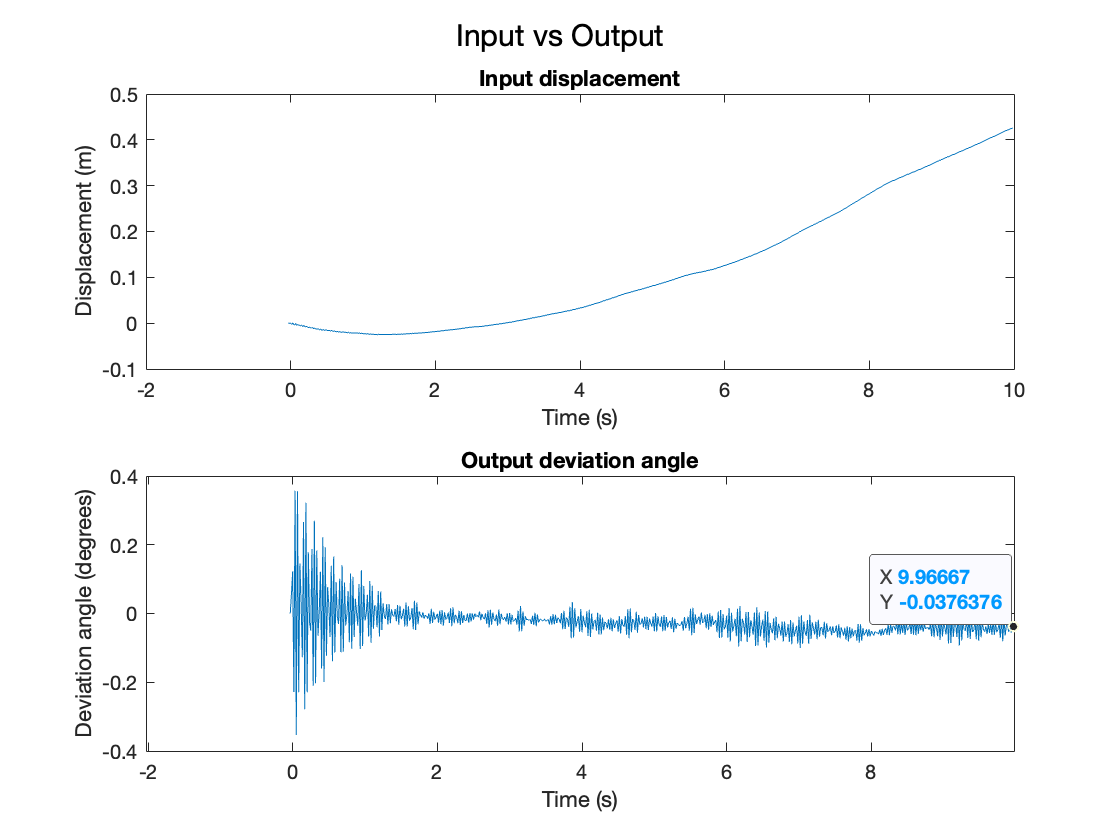
\includegraphics[scale=0.35]{images/PID.png}
    \caption{ PID controller output }
    \label{fig:PID}
\end{figure}

\pagebreak

\begin{figure}[h!]
    \centering
    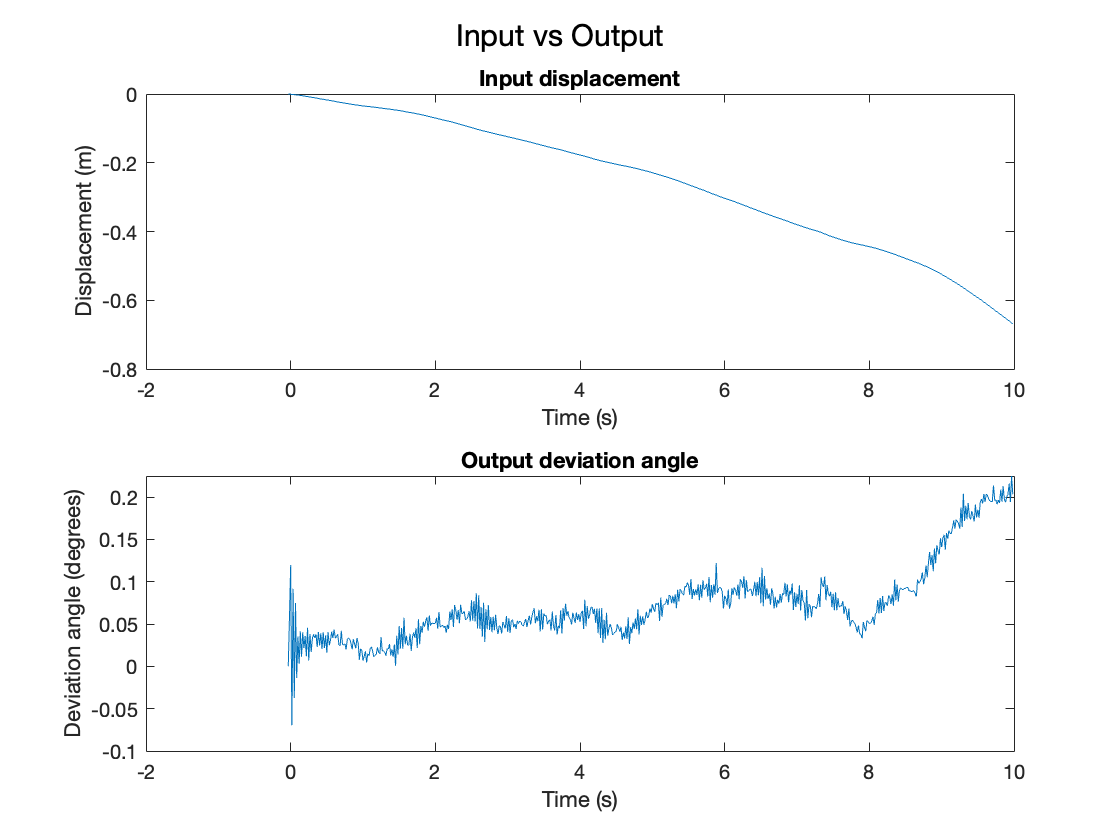
\includegraphics[scale=0.35]{images/FLC.png}
    \caption{ FLC output }
    \label{fig:FLC}
\end{figure}

It is to be noted that with disturbances, both controllers often struggle to bring the pendulum back to the zero position. However, both controllers are able to stabilize the system with reasonable degree of success, though not nearly sufficient for industrial use.


\section{Conclusions}

Since the PID controller takes action while factoring 3 different facets of the deviation angle, it outperforms our current fuzzy controller. We will need to upgrade our fuzzy controller if we want it to compete. Overall, we need to design the Control Action vs $\phi$ curve better. The things we could do to achieve this include
\begin{enumerate}
	\item Increase the number of sets we can classify the state into
	\item Select the control action values better
	\item Consider multiple facets of the error, such as the integral and derivative as well
	\item Use a different class of membership functions
\end{enumerate}

Another thing we could do is to get the best of both worlds by implementing a form of fuzzy PID control. 

\section{Learning Outcomes}

We learnt how to model simple systems on MATLAB, be it linear or non-linear. We learnt how to stabilize unstable systems with both PID and fuzzy logic control. All three of us were new to fuzzy logic, and in general learnt a lot about how things work. Though we didn't get to implement everything that we learnt, we learnt a lot through this project. \\

Things we were looking forward to learn but couldn't due to time constraints include standard techniques for tuning PID for unstable systems, how to design fuzzy logic controllers properly for such systems, and multi-input fuzzy logic controllers for the same. Advanced topics that we only glanced at include adaptive or fuzzy PID controllers, and neural networks for the control of such systems. 
\section{Future Scope}

The study in general could be improved by introducing metrics for the evaluation of the different controllers considered. Towards the end, we realized that our work is too qualitative. \\

Similarly, the study can be improved by designing the PID and FL controllers more rigorously. For the PID controllers, tuning could be done by employing genetic algorithms, or even by optimally solving for the controller transfer function. We realized towards the end that we had enough information for doing so. \\

As for the Fuzzy Logic Controllers, they could be improved by choosing all the parameters more carefully. The parameters include the number of sets defined, the membership functions' widths and shapes. The parameters could have been selected better if the big picture was kept in mind. In general, the FLC could have been designed with more inputs, such as the rate of change of error, or the accumulation of the error in the output. \\
\section{Contributions}

The project was undertaken by Sashank Krishna S, Satwik Vats and Aryan Balyan. Sashank wrote the MATLAB scripts and a significant portion of the report, while Satwik and Aryan worked on making the presentation and helped with debugging some of the scripts. Overall, the work split would be as follows:
\begin{center}
\begin{tabular}{ | c | c | }
	\hline
	Sashank Krishna S 	& 	60 \% \\
	\hline
	Satwik Vats 		& 	20 \% \\  
	\hline
	Aryan Balyan		&	20 \% \\
	\hline
\end{tabular}
\end{center}



\section{Acknowledgements}

I would like to thank Dr. Puneet Mishra and Dr. Surekha Bhanot for teaching the Industrial Instrumentation and Control course, without which this study would not have been possible.

\printbibliography[heading=bibnumbered]

\end{document}

